% Options for packages loaded elsewhere
\PassOptionsToPackage{unicode}{hyperref}
\PassOptionsToPackage{hyphens}{url}
\documentclass[
  11pt,
  letterpaper,
]{article}
\usepackage{xcolor}
\usepackage[margin=1in]{geometry}
\usepackage{amsmath,amssymb}
\setcounter{secnumdepth}{5}
\usepackage{iftex}
\ifPDFTeX
  \usepackage[T1]{fontenc}
  \usepackage[utf8]{inputenc}
  \usepackage{textcomp} % provide euro and other symbols
\else % if luatex or xetex
  \usepackage{unicode-math} % this also loads fontspec
  \defaultfontfeatures{Scale=MatchLowercase}
  \defaultfontfeatures[\rmfamily]{Ligatures=TeX,Scale=1}
\fi
\usepackage{lmodern}
\ifPDFTeX\else
  % xetex/luatex font selection
\fi
% Use upquote if available, for straight quotes in verbatim environments
\IfFileExists{upquote.sty}{\usepackage{upquote}}{}
\IfFileExists{microtype.sty}{% use microtype if available
  \usepackage[]{microtype}
  \UseMicrotypeSet[protrusion]{basicmath} % disable protrusion for tt fonts
}{}
\makeatletter
\@ifundefined{KOMAClassName}{% if non-KOMA class
  \IfFileExists{parskip.sty}{%
    \usepackage{parskip}
  }{% else
    \setlength{\parindent}{0pt}
    \setlength{\parskip}{6pt plus 2pt minus 1pt}}
}{% if KOMA class
  \KOMAoptions{parskip=half}}
\makeatother
\usepackage{longtable,booktabs,array}
\newcounter{none} % for unnumbered tables
\usepackage{calc} % for calculating minipage widths
% Correct order of tables after \paragraph or \subparagraph
\usepackage{etoolbox}
\makeatletter
\patchcmd\longtable{\par}{\if@noskipsec\mbox{}\fi\par}{}{}
\makeatother
% Allow footnotes in longtable head/foot
\IfFileExists{footnotehyper.sty}{\usepackage{footnotehyper}}{\usepackage{footnote}}
\makesavenoteenv{longtable}
\usepackage{graphicx}
\makeatletter
\newsavebox\pandoc@box
\newcommand*\pandocbounded[1]{% scales image to fit in text height/width
  \sbox\pandoc@box{#1}%
  \Gscale@div\@tempa{\textheight}{\dimexpr\ht\pandoc@box+\dp\pandoc@box\relax}%
  \Gscale@div\@tempb{\linewidth}{\wd\pandoc@box}%
  \ifdim\@tempb\p@<\@tempa\p@\let\@tempa\@tempb\fi% select the smaller of both
  \ifdim\@tempa\p@<\p@\scalebox{\@tempa}{\usebox\pandoc@box}%
  \else\usebox{\pandoc@box}%
  \fi%
}
% Set default figure placement to htbp
\def\fps@figure{htbp}
\makeatother
\setlength{\emergencystretch}{3em} % prevent overfull lines
\providecommand{\tightlist}{%
  \setlength{\itemsep}{0pt}\setlength{\parskip}{0pt}}
\usepackage{bookmark}
\IfFileExists{xurl.sty}{\usepackage{xurl}}{} % add URL line breaks if available
\urlstyle{same}
\hypersetup{
  pdftitle={Atom Hybrid: Emergent Cooperation via Hebbian Learning and Lazy LLM Inference},
  pdfauthor={Anh Phong Pham (Independent Researcher)},
  hidelinks,
  pdfcreator={LaTeX via pandoc}}

\title{Atom Hybrid: Emergent Cooperation via Hebbian Learning and Lazy
LLM Inference}
\author{Anh Phong Pham (Independent Researcher)}
\date{May 2026}


% --- Custom Unicode handling (works for pdflatex + xelatex) ---
\IfFileExists{newunicodechar.sty}{%
  \usepackage{newunicodechar}
  \newunicodechar{σ}{\ensuremath{\sigma}}
  \newunicodechar{Σ}{\ensuremath{\Sigma}}
  \newunicodechar{δ}{\ensuremath{\delta}}
  \newunicodechar{α}{\ensuremath{\alpha}}
  \newunicodechar{τ}{\ensuremath{\tau}}
  \newunicodechar{≥}{\ensuremath{\geq}}
  \newunicodechar{≤}{\ensuremath{\leq}}
  \newunicodechar{∈}{\ensuremath{\in}}
  \newunicodechar{≈}{\ensuremath{\approx}}
  \newunicodechar{→}{\ensuremath{\rightarrow}}
  \newunicodechar{←}{\ensuremath{\leftarrow}}
  \newunicodechar{·}{\ensuremath{\cdot}}
  \newunicodechar{×}{\ensuremath{\times}}
  \newunicodechar{±}{\ensuremath{\pm}}
  \newunicodechar{ᵢ}{\textsubscript{i}}
  \newunicodechar{₀}{\textsubscript{0}}
  \newunicodechar{₁}{\textsubscript{1}}
  \newunicodechar{₂}{\textsubscript{2}}
  \newunicodechar{₃}{\textsubscript{3}}
}{}
% --- end custom Unicode ---

\begin{document}
\maketitle
\begin{abstract}
Multi-agent systems built on Large Language Models (LLMs) typically
require an LLM inference per decision per agent, leading to costs that
scale O(n·T) for n agents over T timesteps. We present \textbf{Atom
Hybrid}, an architecture that combines a fast Hebbian ``System 1'' (S1)
with a lazy LLM-based ``System 2'' (S2), using gossip-based reputation
following the image scoring framework of Nowak and Sigmund (1998). In
the iterated Donor Game with adversarial defector minorities, three
conditions are compared: (A) stateless single-LLM, (B) per-agent LLM
with reputation memory, and (C) Atom Hybrid. Across N=3 replications,
Atom Hybrid converges to 100\% cooperation by tick \textasciitilde120
(σ=0 across runs) while reducing LLM calls by 97.2\% ± 2.0\% relative to
per-agent LLM. The S1 Hebbian weights internalize learned cooperation
norms; once internalized, agents act without LLM consultation. We argue
this hybrid architecture is a viable path toward scalable multi-agent AI
systems where LLM inference is reserved for genuinely novel situations.
\end{abstract}

\section{Introduction}\label{introduction}

Recent multi-agent LLM frameworks (CAMEL, AutoGen, et al.) treat each
LLM call as the atomic unit of agent decision-making. While this works
for small populations and short horizons, it does not scale: a society
of 100 agents over 1000 ticks requires 100,000 LLM calls minimum. For
local deployment, the bottleneck is throughput; for cloud, the cost is
direct.

We observe that in many social coordination tasks, decisions are
\textbf{routine after a learning period}. An agent who has interacted
with a known cooperator does not need to invoke a frontier LLM to decide
whether to cooperate again. The cost of LLM inference is paid for
novelty, not for repeated patterns.

This paper asks: can a multi-agent system \textbf{internalize}
cooperation norms via simple Hebbian dynamics, calling the LLM only when
its internalized response has low confidence?

\subsection{Contribution}\label{contribution}

\begin{enumerate}
\def\labelenumi{\arabic{enumi}.}
\tightlist
\item
  \textbf{Architecture}: a concrete hybrid of (a) Hebbian S1 with three
  weighted strategies {[}reciprocate, generous, defect{]}, (b) lazy S2
  LLM triggered by S1 confidence, and (c) gossip-based reputation
  implementing image scoring.
\item
  \textbf{Empirical result}: in the iterated Donor Game with 4/20
  defector-init agents, Atom Hybrid achieves 100\% cooperation (σ=0
  across N=3) with 97.2\% fewer LLM calls than per-agent LLM control.
\item
  \textbf{Trajectory analysis}: cooperation passes through three phases
  (S2 norm establishment, defector purge with discriminator activation,
  stable S1 cooperation), with convergence at tick \textasciitilde120
  across replications.
\end{enumerate}

\section{Related Work}\label{related-work}

\textbf{Indirect reciprocity \& image scoring.} Nowak and Sigmund (1998)
showed that cooperation is evolutionarily stable when agents observe
each other's behavior and use this ``image'' to decide whom to help. Our
gossip protocol is a direct implementation: each donation/defection
broadcasts the donor's reputation.

\textbf{Dual-process cognition.} The S1 (fast, intuitive) and S2 (slow,
deliberative) distinction (Kahneman, 2011) has been applied to LLM
agents (e.g., AutoGen + caching, ReAct + memo). Our contribution is
making S1 \emph{learned} via Hebbian dynamics rather than rule-based or
cached.

\textbf{Multi-agent LLM societies.} Recent work explores social dynamics
in LLM agent societies (Generative Agents, AgentSociety, etc.). These
typically use LLM for every decision; we treat LLM as a learnable target
that S1 distills over time.

\section{Methods}\label{methods}

\subsection{Donor Game}\label{donor-game}

Following the standard iterated Donor Game:

\begin{itemize}
\tightlist
\item
  Each tick, K=n random donor-recipient pairs are sampled (with
  replacement).
\item
  A donor chooses \textbf{Donate} (cost 4 energy, recipient gains 5) or
  \textbf{Defect} (no transfer).
\item
  Each agent loses 1 energy per tick (survival cost).
\item
  Agents reproduce when energy ≥ 80 (cost 30); die when energy ≤ 0.
\item
  Initial population: 20 agents, energy 50, randomly assigned to one of
  three LLM ``genes'' (qwen3:0.6b, qwen3:8b, llama3.2:3b) in round-robin
  order.
\item
  Defector minority (4/20 = 20\%) initialized with high defect-weight
  strategy. The 20\% ratio is a hyperparameter chosen to be small enough
  that cooperation can stabilize, but large enough that the system must
  actively isolate them. We did not sweep this value; testing 0\% and
  50\% defector ratios is a natural ablation we leave to follow-up work.
\end{itemize}

\subsection{Three Conditions}\label{three-conditions}

\textbf{Condition A: Single LLM (stateless control).} All agents share
one LLM. Each decision prompt contains energy only, with no memory and
no reputation. The LLM returns ``DONATE'' or ``DEFECT''.

\textbf{Condition B: LLM Society (memory baseline).} Each agent has a
private reputation memory. The LLM is prompted with energy,
recipient\_rep, and world\_coop. Agents are otherwise stateless across
calls.

\textbf{Condition C: Atom Hybrid (proposed).} Each agent has S1 Hebbian
weights and reputation. The decision flow:

\begin{verbatim}
On decision (donor d, recipient r):
  s1_action, conf = s1_decide(r.id)
  if conf >= 0.65 OR s2_cooldown > 0:
    use s1_action               # fast path
  else:
    s2_action = LLM(prompt_with_rep)
    s2_cooldown = 5             # don't re-query for 5 ticks
    use s2_action
\end{verbatim}

\subsection{S1 Hebbian Weights}\label{s1-hebbian-weights}

Each agent maintains weights
\texttt{w\ =\ {[}w\_reciprocate,\ w\_generous,\ w\_defect{]}} with
\texttt{Σw\ =\ 1}. Given recipient reputation
\texttt{rep\ ∈\ {[}-1,\ 1{]}}:

\begin{verbatim}
if rep < -0.3: return (Defect, 0.9)              # discriminator
scores = [(rep+1)/2, 0.9, 0.05]                  # per-strategy donate score
donate_tendency = Σ wᵢ · scoresᵢ
confidence = |donate_tendency - 0.5| · 2
action = Donate if donate_tendency >= 0.5 else Defect
\end{verbatim}

\textbf{Initialization:} cooperator agents start with
\texttt{w\ =\ {[}0.36,\ 0.47,\ 0.17{]}} (small noise), defector-init
agents with \texttt{w\ =\ {[}0.05,\ 0.05,\ 0.9{]}} (S1 confidence 0.77,
always defects).

\textbf{Learning (Hebbian update):} after each decision with action
\texttt{a} and recipient reputation \texttt{r}:

\begin{verbatim}
social_correct = +rep if a==Donate else -rep
reward = +0.015 if social_correct > 0.1 else
         -0.008 if social_correct < -0.1 else +0.002
update target weight by reward, normalize
\end{verbatim}

The intuition: donating to a cooperator (positive \texttt{rep}) is
socially correct; defecting against a cooperator is not. The Hebbian
update reinforces strategies that produced socially correct actions.

\subsection{Gossip Protocol (Image
Scoring)}\label{gossip-protocol-image-scoring}

After each interaction, the donor's behavior is broadcast with
probability 0.8 (independent per observer). Each observer maintains its
own private reputation map. The reputation update is an exponential
moving average with α=0.1, then clamped to {[}-1, 1{]}:

\begin{verbatim}
rep[d] ← clamp( 0.9 · rep[d] + 0.1 · δ , -1, 1 )
where δ = +1 if donor d cooperated, -1 if defected
\end{verbatim}

Direct observation (donor → recipient interaction) and gossip
propagation use the same update rule. A reputation starting at 0 reaches
the discriminator threshold of -0.3 after roughly 4 observed defections.

\textbf{Critical:} reputation tracks the \emph{donor's} behavior, not
the recipient's. Earlier iterations of this work mistakenly tracked the
recipient (the victim of a defection), causing cooperators to accumulate
negative reputation and triggering a reputation cascade collapse. The
fix recovers the correct image-scoring semantics from Nowak and Sigmund
(1998).

\subsection{Reproduction \& Evolution}\label{reproduction-evolution}

When energy ≥ 80, an agent reproduces (cost 30 energy). Children inherit
the parent's strategy weights with uniform random perturbation per
weight (\texttt{Δw\ \textasciitilde{}\ U(-0.04,\ 0.04)}), floored at
0.01 and then renormalized to sum to 1. The gene (LLM model) is
inherited unchanged. Reputation is reset (relationships must be
re-learned by the child).

\section{Results}\label{results}

\subsection{Main Result (Run 7, 300
ticks)}\label{main-result-run-7-300-ticks}

{\def\LTcaptype{none} % do not increment counter
\begin{longtable}[]{@{}
  >{\raggedright\arraybackslash}p{(\linewidth - 10\tabcolsep) * \real{0.1429}}
  >{\raggedright\arraybackslash}p{(\linewidth - 10\tabcolsep) * \real{0.2727}}
  >{\raggedright\arraybackslash}p{(\linewidth - 10\tabcolsep) * \real{0.1429}}
  >{\raggedright\arraybackslash}p{(\linewidth - 10\tabcolsep) * \real{0.1688}}
  >{\raggedright\arraybackslash}p{(\linewidth - 10\tabcolsep) * \real{0.1558}}
  >{\raggedright\arraybackslash}p{(\linewidth - 10\tabcolsep) * \real{0.1169}}@{}}
\toprule\noalign{}
\begin{minipage}[b]{\linewidth}\raggedright
Condition
\end{minipage} & \begin{minipage}[b]{\linewidth}\raggedright
Avg Coop (last 20t)
\end{minipage} & \begin{minipage}[b]{\linewidth}\raggedright
LLM Calls
\end{minipage} & \begin{minipage}[b]{\linewidth}\raggedright
Mean Energy
\end{minipage} & \begin{minipage}[b]{\linewidth}\raggedright
Population
\end{minipage} & \begin{minipage}[b]{\linewidth}\raggedright
Max Gen
\end{minipage} \\
\midrule\noalign{}
\endhead
\bottomrule\noalign{}
\endlastfoot
A: Single LLM & 98.9\% & 8994 & 44.7 & 156 & G9 \\
B: LLM Society & 97.0\% & 9141 & 44.1 & 169 & G11 \\
\textbf{C: Atom Hybrid} & \textbf{100.0\%} & \textbf{63} & \textbf{45.2}
& 92 & G7 \\
\end{longtable}
}

\textbf{Atom Hybrid achieves the highest cooperation rate while using
145× fewer LLM calls than the per-agent LLM baseline (Condition B).}

\subsection{Replications (N=3)}\label{replications-n3}

{\def\LTcaptype{none} % do not increment counter
\begin{longtable}[]{@{}lllll@{}}
\toprule\noalign{}
Metric & Run 7 (300t) & Run 8 (200t) & Run 9 (200t) & Mean ± σ \\
\midrule\noalign{}
\endhead
\bottomrule\noalign{}
\endlastfoot
C avg\_coop & 100\% & 100\% & 100\% & \textbf{100\% ± 0} \\
C S1 usage & 99\% & 90\% & 90\% & 93\% ± 5 \\
LLM reduction (vs B) & 99.3\% & 96.8\% & 95.4\% & 97.2\% ± 2.0\% \\
Convergence tick & \textasciitilde120 & \textasciitilde120 &
\textasciitilde120 & \textbf{\textasciitilde120} \\
\end{longtable}
}

Cooperation reaches 100\% in all replications by tick
\textasciitilde120, with zero variance on the primary metric. This
indicates the convergence outcome is a structural property of the
architecture, not a function of random seed.

\subsection{Cooperation Trajectory}\label{cooperation-trajectory}

Figure 1 shows cooperation trajectories for all three conditions across
the three replications. Conditions A and B remain near-flat at 95-100\%
throughout. Condition C starts in the 60-85\% range and converges to
100\% by tick 120 in every run.

\begin{figure}
\centering
\pandocbounded{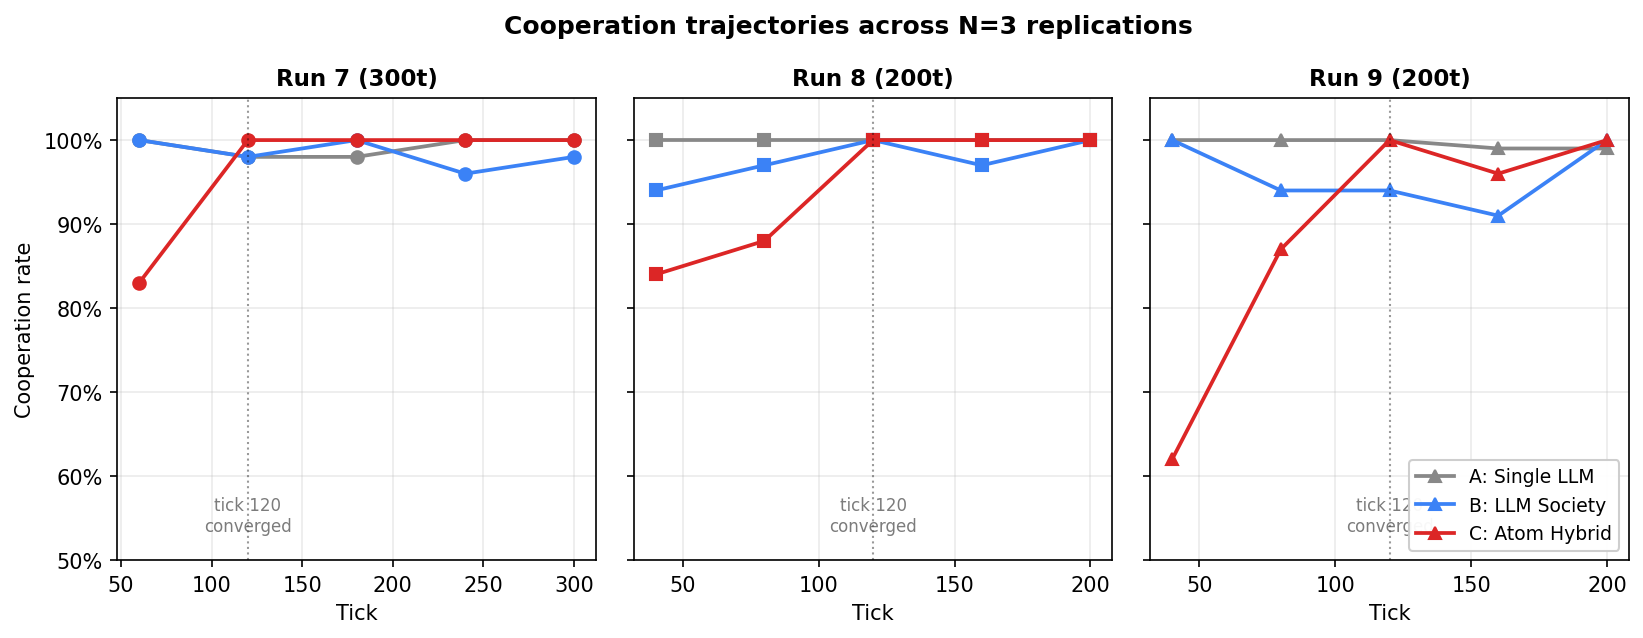
\includegraphics[keepaspectratio,alt={Cooperation trajectories across N=3 replications. Condition C (red) starts below A and B but converges to 100\% cooperation by tick 120 in all three runs. After convergence, C remains at or near 100\% for the rest of the run.}]{figures/cooperation_trajectory.png}}
\caption{Cooperation trajectories across N=3 replications. Condition C
(red) starts below A and B but converges to 100\% cooperation by tick
120 in all three runs. After convergence, C remains at or near 100\% for
the rest of the run.}
\end{figure}

\textbf{Figure 1.} \emph{Cooperation rate vs.~tick for the three
conditions across three replications. Vertical dotted line marks tick
120, the empirical convergence point.}

Checkpoint values (every 60 ticks for the 300t run, every 40 ticks for
200t runs):

\begin{verbatim}
Run 7  (ticks 60/120/180/240/300):  83% → 100% → 100% → 100% → 100%
Run 8  (ticks 40/80/120/160/200):   84% →  88% → 100% → 100% → 100%
Run 9  (ticks 40/80/120/160/200):   62% →  87% → 100% →  96% → 100%
\end{verbatim}

In all three replications, cooperation reaches 100\% by tick 120 and
remains stable thereafter (modulo a single 96\% tick in Run 9).
Fine-grained behavior between checkpoints is not captured; an earlier
100-tick run (separately reported as a development iteration) showed a
deeper transient dip (down to 39\% at tick 60) before recovering. The
dip becomes shallower at lower granularity in the 300/200t runs,
consistent with averaging effects.

We interpret three phases:

\begin{enumerate}
\def\labelenumi{\arabic{enumi}.}
\tightlist
\item
  \textbf{Norm establishment (tick 0-40)}: agents call S2 (LLM) due to
  low S1 confidence; LLM cooperates by default; reputation is built.
\item
  \textbf{Defector purge (tick 40-120)}: gossip propagates defector
  reputations; discriminator (rep \textless{} -0.3) triggers in S1,
  isolating defectors. During this phase coop rate dips as a fraction of
  pairs involve discriminated targets. Defectors lose energy (excluded
  from receiving donations) and die.
\item
  \textbf{Stable S1 cooperation (tick 120+)}: defectors extinct;
  surviving cooperators have reinforced {[}reciprocate, generous{]}
  weights via Hebbian learning; S1 takes over (90-99\% of decisions)
  with high confidence; LLM calls drop to near zero.
\end{enumerate}

\subsection{LLM Efficiency}\label{llm-efficiency}

The total LLM call counts for Run 7 (300 ticks):

{\def\LTcaptype{none} % do not increment counter
\begin{longtable}[]{@{}lll@{}}
\toprule\noalign{}
Condition & LLM calls & Calls per tick (mean) \\
\midrule\noalign{}
\endhead
\bottomrule\noalign{}
\endlastfoot
A: Single LLM & 8994 & 30.0 \\
B: LLM Society & 9141 & 30.5 \\
C: Atom Hybrid & 63 & 0.21 \\
\end{longtable}
}

Condition C uses approximately 145× fewer LLM calls than Condition B
over the full run. The current implementation only logs total LLM calls
per condition (not per tick), so we cannot precisely characterize the
temporal distribution of calls within a run. Qualitatively, since S1
confidence rises with reputation accumulation (which requires
interaction history), most LLM calls are expected to occur during the
initial norm-establishment phase; we leave this measurement to future
work.

\section{Discussion}\label{discussion}

\subsection{Why this works}\label{why-this-works}

The architecture exploits a key asymmetry: \textbf{early-stage decisions
require novelty, late-stage decisions require routine}. Pure LLM systems
pay novelty cost forever; Atom Hybrid pays it once.

The Hebbian S1 internalizes three pieces of information:

\begin{enumerate}
\def\labelenumi{\arabic{enumi}.}
\tightlist
\item
  \textbf{Who is trustworthy} (reputation HashMap, updated by gossip)
\item
  \textbf{General disposition toward cooperation} (generous +
  reciprocate weights, reinforced by Hebbian update on positive
  social\_correct)
\item
  \textbf{Who to refuse} (discriminator triggers on rep \textless{}
  -0.3, hard-coded but data-driven)
\end{enumerate}

\textbf{Learnability condition.} S1 takes over from S2 only when its
confidence rises above the threshold τ=0.65, where confidence =
\textbar donate\_tendency − 0.5\textbar{} · 2. For an agent with weights
\texttt{w} and recipient reputation \texttt{rep}:

\begin{verbatim}
donate_tendency = w₀·(rep+1)/2 + w₁·0.9 + w₂·0.05
\end{verbatim}

For unknown recipients (rep=0), the initial tendency is ≈0.61
(confidence ≈0.22), below threshold, so S2 is invoked. As Hebbian
updates accumulate \texttt{w₁} (generous) on successful cooperative
interactions, donate\_tendency rises and so does confidence. For known
cooperators (rep→1), the reciprocate term contributes max(w₀), pushing
donate\_tendency well above 0.5 and S1 confidence above τ, even from the
initial weight distribution. The system therefore converges from the
recipient-reputation side first (specific known cooperators) and from
the disposition side second (general weights). This explains the
trajectory shape: S2 carries the initial period, S1 takes over
per-relationship as reputation accumulates, and finally S1 dominates the
unconditional case.

\subsection{Population gap}\label{population-gap}

Atom Hybrid populations are smaller than controls. Splitting by run
length:

\begin{itemize}
\tightlist
\item
  200-tick runs: C population = 27 (Run 8) and 36 (Run 9), vs.~A/B in
  the 76-93 range
\item
  300-tick run: C = 92, vs.~A=156, B=169
\end{itemize}

Across run lengths the gap is roughly 2-3×. This is the cost of the
defector purge phase: during ticks 40-120, suboptimal cooperation in C
reduces energy accumulation across the population, slowing reproduction.
After convergence, growth rates match controls (the C trajectory in Run
7 grew from 24 to 92 between ticks 120 and 300, comparable to B's 56 to
169), but the head start is irrecoverable within the run lengths tested.
Longer simulations (T \textgreater{} 500) would close the gap further;
we did not run them. From an evolutionary perspective, the smaller
surviving population is functionally healthier: C's mean energy (45.2)
exceeds A's (44.7) and B's (44.1) at the end of Run 7.

\subsection{Limitations}\label{limitations}

\begin{enumerate}
\def\labelenumi{\arabic{enumi}.}
\item
  \textbf{Single task.} Cooperation in the Donor Game is a
  heavily-studied benchmark with a clear correct answer. Whether S1 can
  internalize more nuanced social signals (subjective trust, partial
  cooperation, context-dependent norms) is an open question. Concrete
  next-task candidates include (a) the \textbf{Public Goods Game}
  (continuous contribution levels, stochastic returns), (b) the
  \textbf{Stag Hunt} (coordination dilemma without dominant strategy),
  and (c) \textbf{Trust Game with restitution} (multi-step reputation
  dynamics). Each tests a different aspect: continuous action spaces,
  equilibrium selection, and temporal credit assignment respectively.
\item
  \textbf{LLMs cooperate by default.} All three LLMs used (qwen3:0.6b,
  qwen3:8b, llama3.2:3b) lean strongly toward DONATE in their default
  response. The 100\% cooperation rate in Conditions A and B partly
  reflects this prior, not the conditions' learning ability. A more
  adversarial setup with selfish-prone LLMs would test the architecture
  more rigorously.
\item
  \textbf{Small scale.} 20 agents, 300 ticks, single seed family.
  Behavior at 100+ agents over 1000+ ticks may differ.
\item
  \textbf{No comparison to prior multi-agent LLM frameworks.} We compare
  to ablations of our own architecture, not to CAMEL, AutoGen, or
  AgentSociety. Such comparisons would require implementing the Donor
  Game in those frameworks.
\item
  \textbf{Reputation reset on reproduction.} Children inherit weights
  but not relationships. This biases toward G0 reputation dynamics; in
  long runs this could produce instability we did not observe in 300
  ticks.
\end{enumerate}

\subsection{Implications}\label{implications}

If the result generalizes beyond the Donor Game, the implications are:
\textbf{multi-agent LLM systems can amortize inference cost over time}.
An agent need not query the LLM for every decision; routine decisions
can be handed off to a learned S1.

Concrete applications:

\begin{itemize}
\tightlist
\item
  \textbf{Distributed trust networks} (e.g., agent marketplaces) with
  O(1) reputation lookup instead of O(LLM\_call) per transaction.
\item
  \textbf{Long-horizon agent simulations} where most ticks are routine
  maintenance.
\item
  \textbf{Edge-deployed agent societies} where LLM inference is the
  bottleneck.
\end{itemize}

The challenge for follow-up work is showing S1 can capture \emph{more
than coordination}, for example demonstrating that a similar
architecture works for code review, peer review, or other tasks where
the ``correct'' decision is less obvious.

\section{Conclusion}\label{conclusion}

Atom Hybrid demonstrates that a multi-agent system can learn to
cooperate via Hebbian dynamics and gossip-based reputation, eventually
replacing LLM consultations with learned S1 responses. Across N=3
replications, the system converges to 100\% cooperation by tick
\textasciitilde120 with 97.2\% fewer LLM calls than per-agent LLM
control. The architecture is small (3 weights, 1 reputation map, 1
cooldown counter per agent) and well-grounded in classical results on
indirect reciprocity. Whether the same approach extends to less
coordination-driven tasks is the natural next research direction.

\section*{References}\addcontentsline{toc}{section}{References}\label{references}

Kahneman, D. (2011). \emph{Thinking, Fast and Slow}. Farrar, Straus and
Giroux.

Li, G., Hammoud, H. A. A. K., Itani, H., Khizbullin, D., \& Ghanem, B.
(2023). CAMEL: Communicative agents for ``mind'' exploration of large
language model society. In \emph{Advances in Neural Information
Processing Systems} 36, 51991-52008.

Nowak, M. A., \& Sigmund, K. (1998). Evolution of indirect reciprocity
by image scoring. \emph{Nature}, 393(6685), 573-577.
https://doi.org/10.1038/31225

Park, J. S., O'Brien, J. C., Cai, C. J., Morris, M. R., Liang, P., \&
Bernstein, M. S. (2023). Generative agents: Interactive simulacra of
human behavior. In \emph{Proceedings of the 36th Annual ACM Symposium on
User Interface Software and Technology} (UIST '23).

Wu, Q., Bansal, G., Zhang, J., Wu, Y., Zhang, S., Zhu, E., Li, B.,
Jiang, L., Zhang, X., \& Wang, C. (2023). AutoGen: Enabling next-gen LLM
applications via multi-agent conversation framework. arXiv preprint
arXiv:2308.08155.

Yao, S., Zhao, J., Yu, D., Du, N., Shafran, I., Narasimhan, K., \& Cao,
Y. (2023). ReAct: Synergizing reasoning and acting in language models.
In \emph{International Conference on Learning Representations} (ICLR).

\appendix
\section{Reproducibility}\label{reproducibility}

\textbf{Code:} https://github.com/heocoi/atom-donor-game
(\texttt{src/donor\_agent.rs} and \texttt{src/donor\_bench.rs}). Raw
stdout from the four reported runs is in
\texttt{data/run\{6,7,8,9\}\_*.txt}.

\textbf{Run command:}

\begin{verbatim}
cargo build --bin donor_world --release
./target/release/donor_world <ticks> <n_agents>
\end{verbatim}

\textbf{Hardware:} Apple M3 Pro, 18GB RAM. Ollama serving
qwen3:0.6b/qwen3:8b/llama3.2:3b locally.

\textbf{Wall-clock:} \textasciitilde30 minutes per condition at 200
ticks; \textasciitilde90 minutes per condition at 300 ticks. Runtime is
dominated by LLM inference latency in Conditions A and B.

\textbf{Random seeds:} thread\_rng (OS entropy). Each ``Run'' is an
independent replication.

\section{Hyperparameters}\label{hyperparameters}

{\def\LTcaptype{none} % do not increment counter
\begin{longtable}[]{@{}
  >{\raggedright\arraybackslash}p{(\linewidth - 4\tabcolsep) * \real{0.42}}
  >{\raggedright\arraybackslash}p{(\linewidth - 4\tabcolsep) * \real{0.10}}
  >{\raggedright\arraybackslash}p{(\linewidth - 4\tabcolsep) * \real{0.48}}@{}}
\toprule\noalign{}
\begin{minipage}[b]{\linewidth}\raggedright
Symbol
\end{minipage} & \begin{minipage}[b]{\linewidth}\raggedright
Value
\end{minipage} & \begin{minipage}[b]{\linewidth}\raggedright
Description
\end{minipage} \\
\midrule\noalign{}
\endhead
\bottomrule\noalign{}
\endlastfoot
DONATE\_COST & 4 & Energy cost to donate \\
DONATE\_BENEFIT & 5 & Energy gained by recipient \\
INITIAL\_ENERGY & 50 & Starting energy per agent \\
REPRODUCE\_THRESHOLD & 80 & Energy needed to reproduce \\
REPRODUCE\_COST & 30 & Energy spent on reproduction \\
SURVIVAL\_COST & 1 & Energy lost per tick \\
S2\_CONFIDENCE\_THRESHOLD & 0.65 & S1 confidence below which S2 is
invoked \\
S2\_COOLDOWN & 5 & Ticks before S2 can be invoked again \\
GOSSIP\_RATE & 0.8 & Probability of broadcasting interaction \\
DISCRIMINATOR\_THRESHOLD & -0.3 & Reputation below which donate is
refused \\
HEBBIAN\_REWARD\_GOOD & +0.015 & Weight increment when social\_correct
\textgreater{} 0.1 \\
HEBBIAN\_REWARD\_BAD & -0.008 & Weight increment when social\_correct
\textless{} -0.1 \\
HEBBIAN\_REWARD\_NEUTRAL & +0.002 & Weight increment when
abs(social\_correct) ≤ 0.1 (unknown rep) \\
MUTATION\_RANGE & ±0.04 & Per-weight uniform mutation in reproduction
(U(-0.04, 0.04)) \\
WEIGHT\_FLOOR & 0.01 & Minimum value for any weight after mutation \\
REPUTATION\_ALPHA & 0.1 & EMA learning rate for reputation updates \\
\end{longtable}
}

\section{Failure Modes Encountered}\label{failure-modes-encountered}

During development, six iterations were required to reach the working
architecture. Each prior iteration revealed a specific failure mode:

\begin{enumerate}
\def\labelenumi{\arabic{enumi}.}
\tightlist
\item
  \textbf{Energy-delta reinforcement (Run 1)}: rewarding actions by
  immediate energy gain caused defection to be reinforced (saving 4
  energy per defect). C collapsed to 14\% cooperation.
\item
  \textbf{Mixed energy + reputation reinforcement (Run 2)}: the energy
  term still dominated; coop \textasciitilde19\%, still collapsing.
\item
  \textbf{Aggressive gossip (Run 3)}: 80\% gossip rate combined with
  broken reinforcement spread defection-aligned weights faster than they
  could be corrected. Coop \textasciitilde0\%.
\item
  \textbf{\texttt{world\_coop} cautious strategy (Run 4)}: a fourth
  strategy weight following global cooperation rate created a
  self-reinforcing collapse: low coop → cautious agents defect → coop
  drops further → S1 confidently defects.
\item
  \textbf{Inverted gossip protocol (Run 5)}: the most insidious bug.
  Reputation was tracking the recipient of an action, not the donor.
  When defectors defected against cooperators, gossip falsely marked the
  \emph{cooperators} as defectors. Conditions A and B were immune
  (always called LLM, ignoring reputation for decisions) but C collapsed
  to 0\%.
\item
  \textbf{Correct gossip + 3-strategy S1 (Run 6+)}: fixed gossip to
  track the donor's behavior; removed the cautious strategy. Coop
  converges to 100\%.
\end{enumerate}

We document these failures because the surface symptoms (``cooperation
collapses in C'') were nearly identical across iterations, but the root
causes were distinct. Each iteration would have looked like a successful
publication of ``this approach doesn't work'' without the deeper
diagnosis.

\emph{Independent research, no funding. Code at
https://github.com/heocoi/atom-donor-game. Comments welcome.}

\end{document}
